\documentclass{beamer}
\usepackage{amsmath}
\usepackage{amsfonts}
\usepackage{amssymb}
\usepackage{polski}
\usepackage{pgfplots}
\pgfplotsset{compat=1.15}
\usepackage{mathrsfs}
\usepackage{wasysym}
\usepackage{booktabs}
\usetikzlibrary{arrows}
\usetheme{Warsaw}
\title{Ile ma Mach, czyli Falentynistyka}

\author{Franciszek Hansdorfer \and Jacek Winiarczyk}
\institute{Wydział fizyki doświadczalnej KFnrD}
\date{\today}
\begin{document}
\begin{frame}
	\titlepage
\end{frame}

\begin{frame}{Co mogą zmierzyć mieszkańcy Falent?}
	\begin{itemize}
		\item $\pi$
		\item $e$
		\item Prędkość dźwięku w powietrzu ($1$ Mach)
		\item Przenikalność magnetyczna próżni ($\epsilon_0$)
		\item Przenikalność elektryczna próżni ($\mu_0$)
		\item Stała Coulomba ($k_e$)
		\item Prędkość światła ($c$)
		\item Stała Plancka ($h$)
		\item Zredukowana stała Plancka ($\hbar$)
	\end{itemize}

\end{frame}

\section{Stałe matematyczne}

\subsection{$\pi$}

\begin{frame}{$\pi$ - igła Buffona}
	$l$ - długość igły

	$d$ - odległość między pionowymi liniami

	$n$ - liczba rzutów

	$R$ - liczba rzutów zakończonych przecięciem

	$$p = \frac{2}{\pi} \frac{l}{d}$$
	$$\frac{R}{n} = \frac{2}{\pi}\frac{l}{d}$$
	$$\pi = \frac{2 l n}{d R}$$
	$$\pi =$$

\end{frame}

\subsection{$e$}

% \begin{frame}{$e$ - całkowanie gumką}

% \end{frame}

\begin{frame}{Czym jest Mach?}

	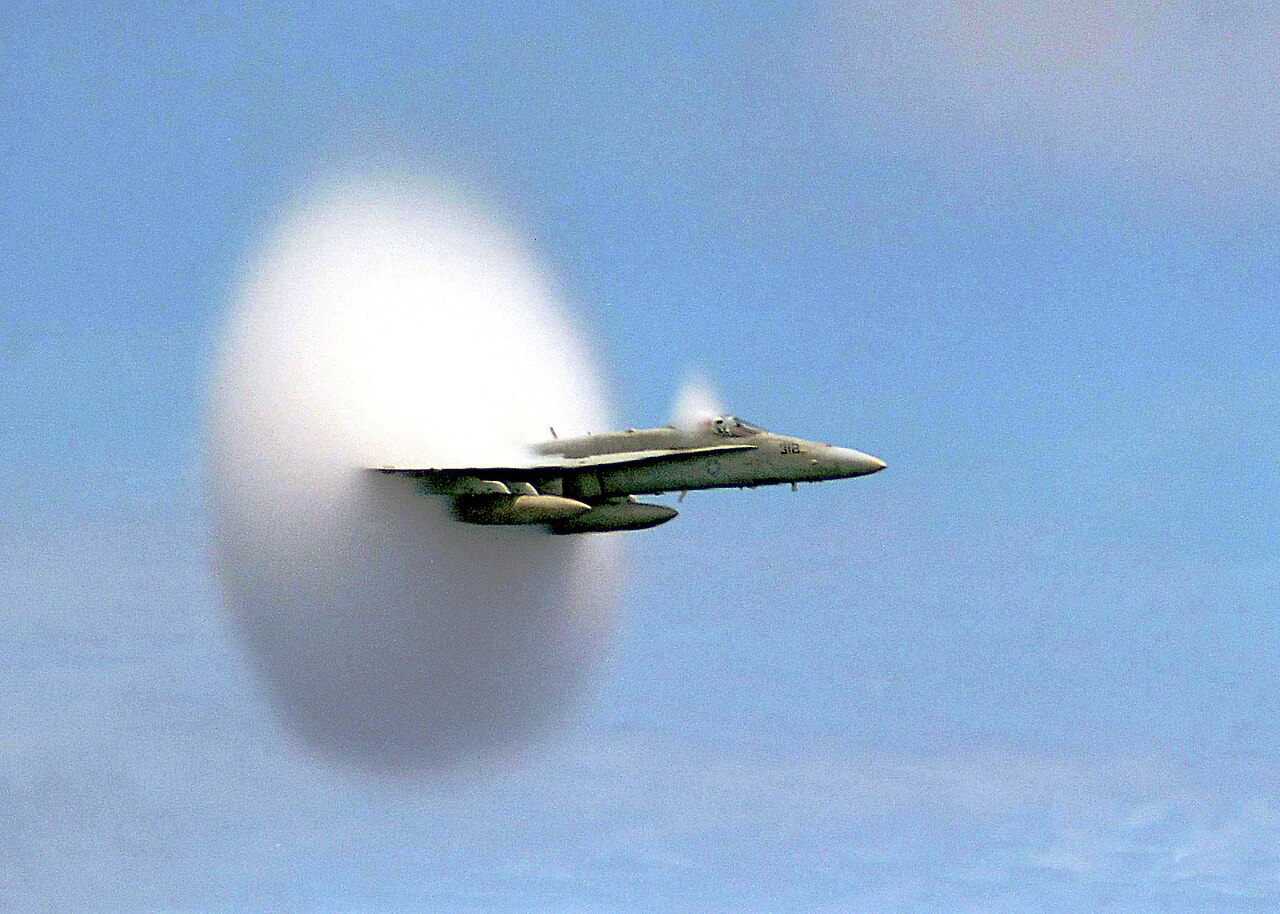
\includegraphics[width=\linewidth]{mach.jpg}

\end{frame}

\section{Parametry fizyczne}

\subsection{Prędkość dźwięku w powietrzu}

\begin{frame}{Prędkość dźwięku w powietrzu}

	\begin{columns}
		\begin{column}{0.5\textwidth}
			Lab:

			\includegraphics[width=\linewidth]{lab_KlaKop.jpg}
		\end{column}
		\begin{column}{0.5\textwidth}
			Aparatura pomiarowa:
			\begin{itemize}
				\item Miarka 3m
				\item Laptop
				\item Dłonie Franka
				\item Dłonie Jacka
				\item Termometr i higrometr
			\end{itemize}
		\end{column}
	\end{columns}

\end{frame}

\subsection{Zasada działania}

\begin{frame}{Zasada działania}

	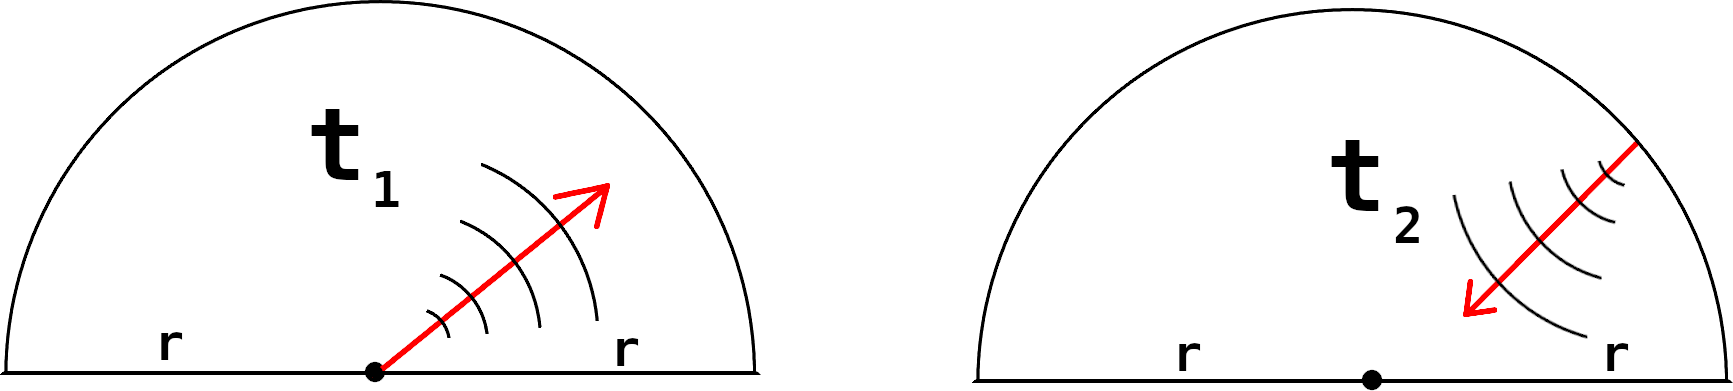
\includegraphics[width=\linewidth]{wave.png}
	$$\Delta t=t_2-t_1$$
	$$v=\frac{2r}{\Delta t}$$

\end{frame}

\begin{frame}{Dane}
	\centering
	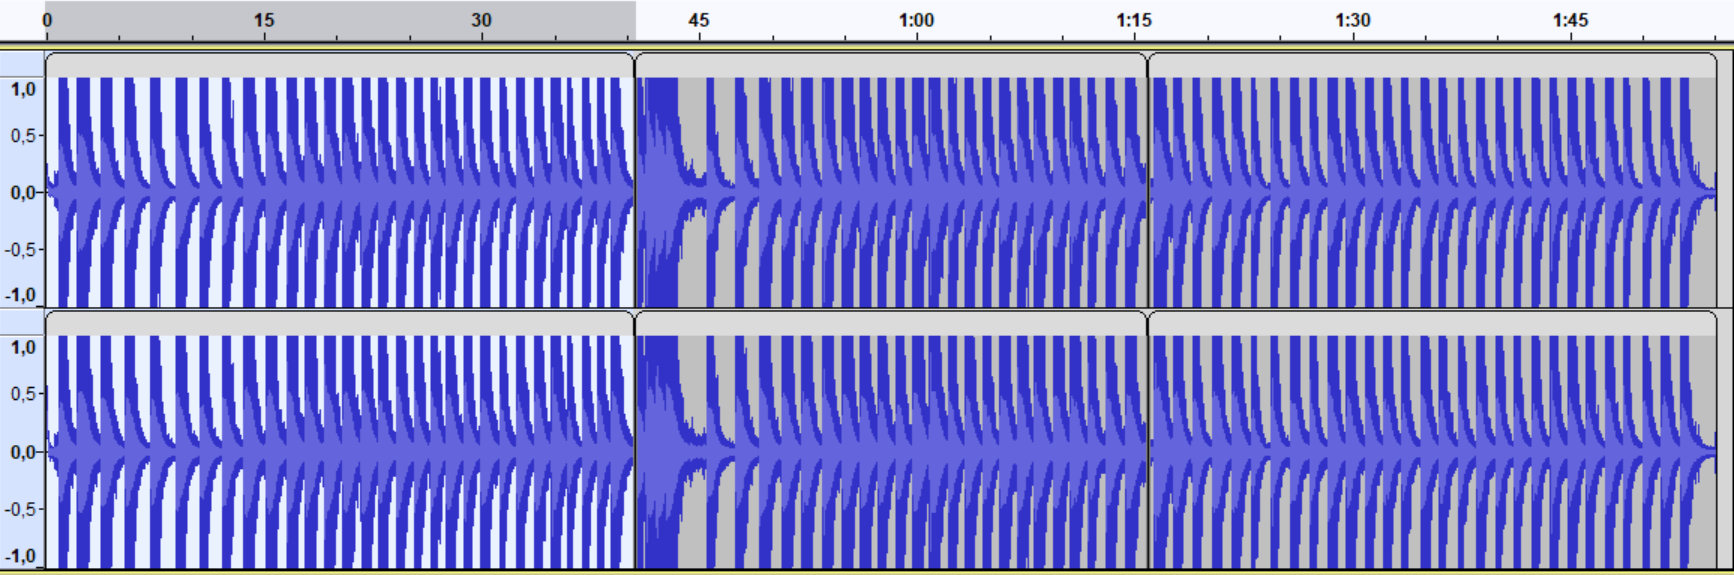
\includegraphics[width=\linewidth]{Data.png}
	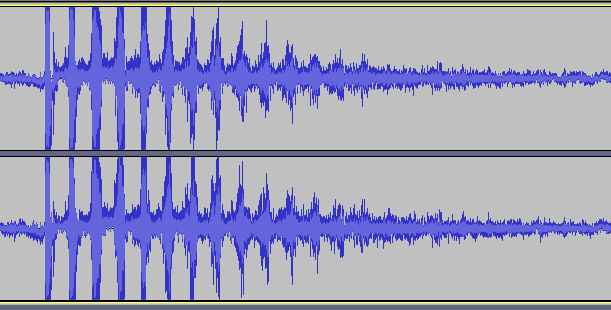
\includegraphics[width=0.7\linewidth]{Przechwycenie obrazu ekranu_2024-05-04_14-41-05.png}
\end{frame}

\begin{frame}{Redukcja danych}
	\centering
	\begin{tabular}{cccc}
		\toprule
		Pomiar & czas [s] & sigma [s] & liczba pomiarów \\
		\midrule
		3      & 0.0534   & 0.00134   & 245             \\
		4      & 0.0533   & 0.00127   & 117             \\
		5      & 0.0544   & 0.00149   & 302             \\
		6      & 0.0548   & 0.00180   & 688             \\
		7      & 0.0550   & 0.00119   & 762             \\
		\bottomrule
	\end{tabular}

	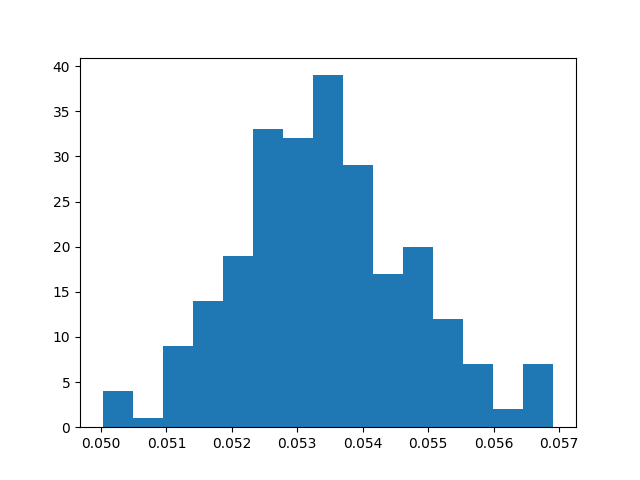
\includegraphics[width=0.2\linewidth]{Hist3.png}
	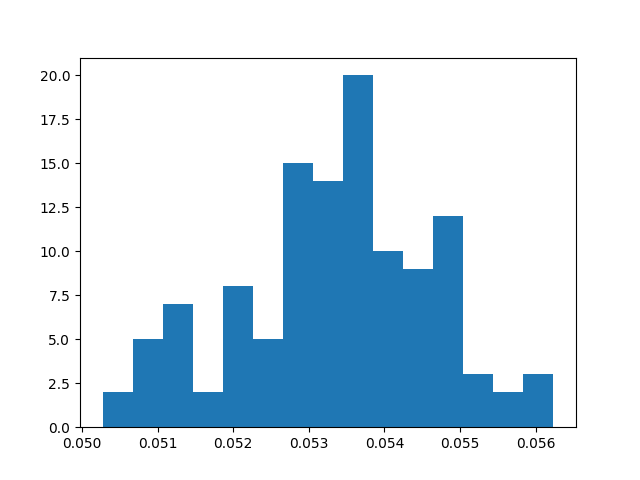
\includegraphics[width=0.2\linewidth]{Hist4.png}
	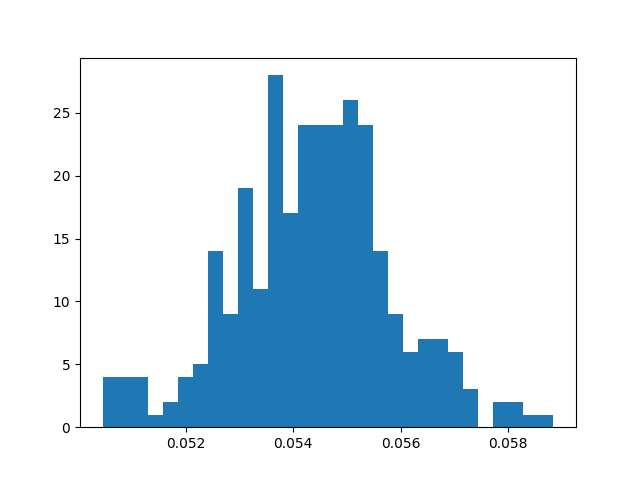
\includegraphics[width=0.2\linewidth]{Hist5.png}
	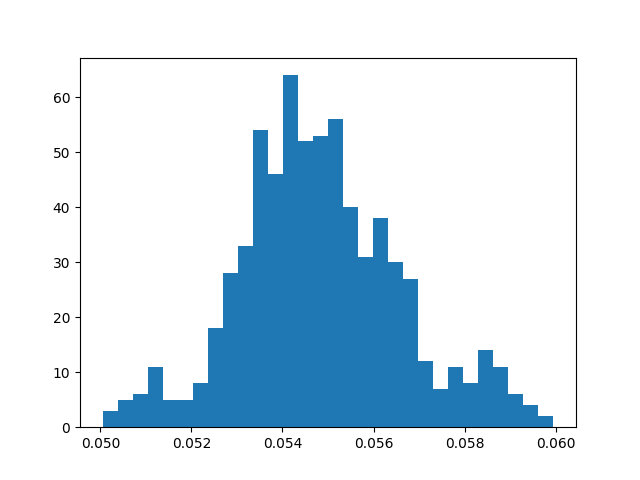
\includegraphics[width=0.2\linewidth]{Hist6.png}
	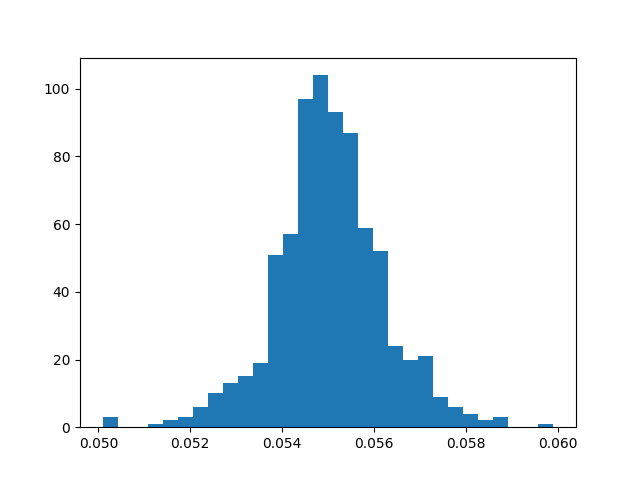
\includegraphics[width=0.2\linewidth]{Hist7.png}
\end{frame}

\begin{frame}{Wyniki i dyskusja błędu pomiarowego}
	\centering
	\begin{tabular}{cccc}
		\toprule
		Pomiar & temperatura [C] & wilgotność [\%] & mach [m/s]       \\
		\midrule
		3      & 29.12           & 27.83           & 355.71$\pm$8.90  \\
		4      & 31.35           & 22.14           & 356.22$\pm$8.51  \\
		5      & 20.22           & 44.42           & 349.41$\pm$9.57  \\
		6      & 18.25           & 51.11           & 346.48$\pm$11.36 \\
		7      & 18.22           & 51.53           & 345.19$\pm$7.46  \\
		\bottomrule
	\end{tabular}

\end{frame}

\begin{frame}{Interpretacja wyników}
	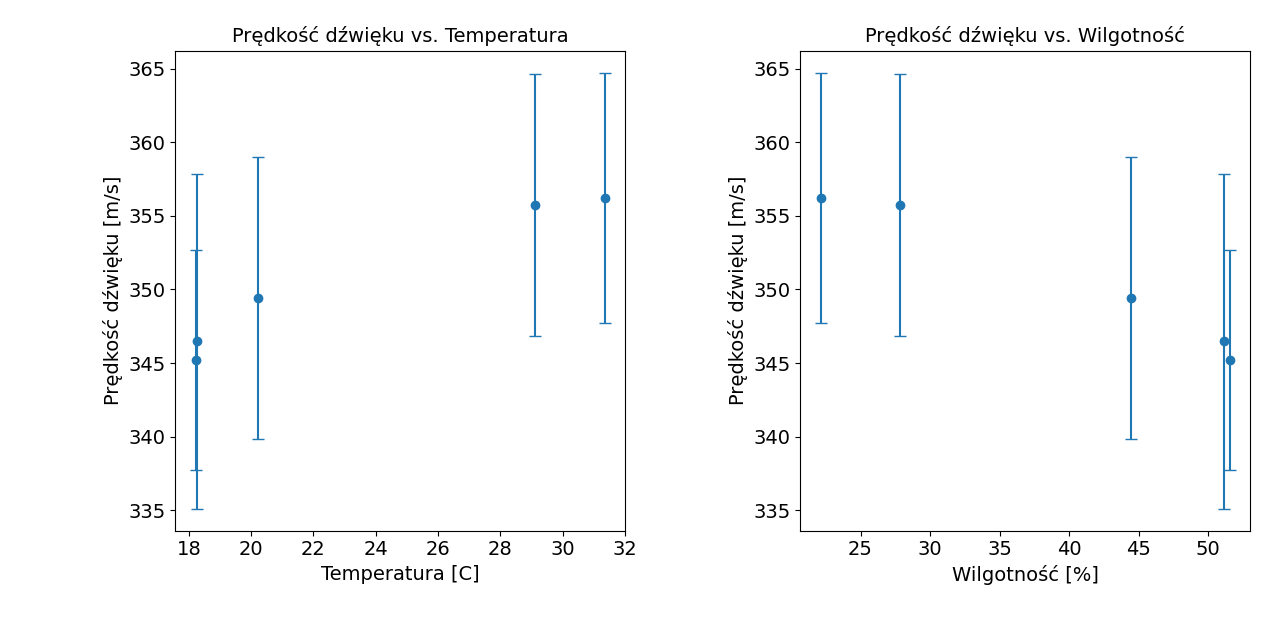
\includegraphics[width=\linewidth]{temp_humid_mach.png}

	Prędkość dźwięku rośnie wraz ze wzrostem temperatury.
\end{frame}


\section{Stałe fizyczne}

\begin{frame}{Przenikalność magnetyczna próżni}
	indukcyjność cewki:
	$$L = \frac{S\mu_0 n^2}{l}$$

	$S$ - pole przekroju cewki
	$\mu_0$ - przenikalność magnetyczna próżni
	$n$- ilość zwojów
	$l$ - długość cewki

	$$\epsilon_c = -L\frac{dI}{dt}$$

\end{frame}

\begin{frame}{Przenikalność magnetyczna próżni}
	$$I = \frac{\epsilon-\epsilon_c}{R}$$

	$$I R = \epsilon + L\frac{dI}{dt}$$
	$$\frac{dI}{dt}\frac{L}{IR-\epsilon}=1$$
	$$L\int\frac{dI}{IR-\epsilon} = \int dt$$
	$$\frac{L}{R}\log(IR-\epsilon) = t+c_1$$
	$$IR - \epsilon = c_2 e^{\frac{Rt}{L}}$$
	$$I = \frac{\epsilon}{R} + c_3 e^{\frac{Rt}{L}}$$

\end{frame}

\begin{frame}
	$$I = \frac{\epsilon}{R} + c_3 e^{\frac{Rt}{L}}$$
	$$I(0)= \frac{\epsilon}{R}$$
	$$I = \frac{\epsilon}{R} + e^{\frac{Rt}{L}}$$
\end{frame}

\begin{frame}{Przenikalność elektryczna próżni}

\end{frame}

\begin{frame}{Stała Plancka}

\end{frame}


\section{Podsumowanie}

\begin{frame}{Dalsze kontynuacje badań}
	\begin{itemize}
		\item Stała Faradaya ($F$)
		\item Ładunek elementarny ($e^-$)
		\item Odległość Ziemia-Księżyc ($d_{\oplus - \leftmoon}$)
		\item Promień Księżyca ($R_{\leftmoon}$)
	\end{itemize}

\end{frame}



\end{document}